\chapter{Wireframes} \label{cha:wireframes}

\section{Hoofdframe} \label{sec:hoofdframe}
\begin{figure}[h]
  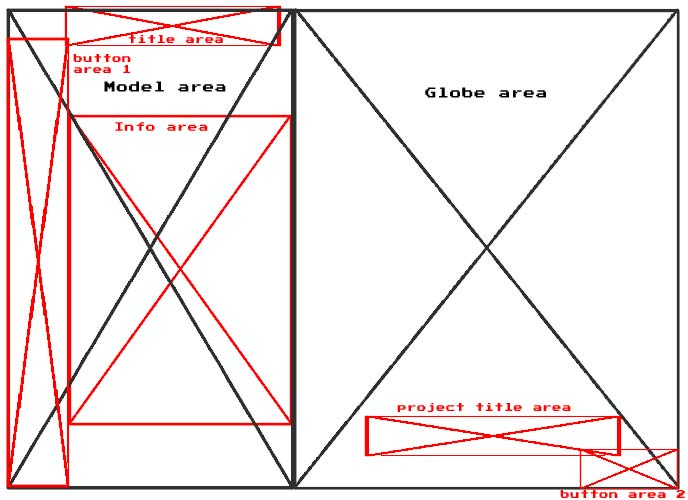
\includegraphics[width=100mm]{figs/wireframe1.jpg}
  \caption{Wireframe 1 \textit{(27-April-2014)}}
  \label{fig:wireframe1}
\end{figure}

De onderste laag is getekend in \textbf{zwart}, de bovenste laag is getekend in het \textbf{{\color{red}rood}}.\\
De \textbf{model area} en \textbf{globe area} zijn de de belangrijkste componenten en bevatten de gehele inhoud van deze applicatie.\\
De \textbf{{\color{red}info area}}, de 2 \textbf{{\color{red}title areas}} en de 2 \textbf{{\color{red}button areas}} zijn altijd zichtbaar boven de andere areas. De \textbf{{\color{red}project title area}} bevat de naam van het project, \projectname\ en de linker \textbf{{\color{red}title area}} bevat de naam van het geselecteerde monument. Vanuit de buttons in \textbf{{\color{red}button area 1}} kan de zichtbaarheid van \textbf{{\color{red}button area 1}} en de \textbf{{\color{red}info area}} worden getoggled. Deze togglebuttons zijn wel altijd zichtbaar. \textbf{{\color{red}button area 2}} en \textbf{{\color{red}project title area}} is ten alle tijden zichtbaar en dient om de applicatie te sluiten.\\
De inhoud van de areas zal in detail worden beschreven in \cref{cha:componenten} \nameref{cha:componenten}.
\newpage
\section{Info area wireframe} \label{sec:infowire}
\begin{figure}[h]
  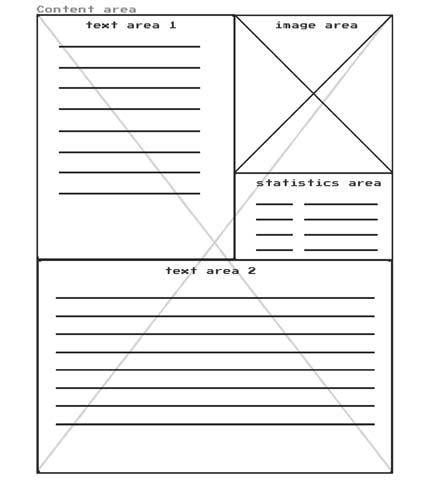
\includegraphics[width=100mm]{figs/wireframe2.jpg}
  \caption{Wireframe 2 (info area)\textit{(27-April-2014)}}
  \label{fig:wireframe2}
\end{figure}

Dit is een uitgewerkte wireframe van de \textbf{info area}. Dit paneel verschijnt als op de button met de letter "i" wordt gedrukt. In de \textbf{{\color{gray}content area}} komt samengevatte informatie te staan. Binnen de \textbf{{\color{gray}content area}} is ruimte voor text, een foto van het monument en enkele statistieken. Deze statistieken zijn gebonden aan het monument, zoals bijvoorbeeld: bouwjaar, architect en locatie gegevens. Een titel voor deze pagina is niet nodig, omdat de titel van het monument nog zichtbaar is in de \textbf{model area}, en geen ander monument kan worden gekozen terwijl het info paneel is geopend.
\newpage
